\documentclass[tikz,10pt]{standalone}

\begin{document}
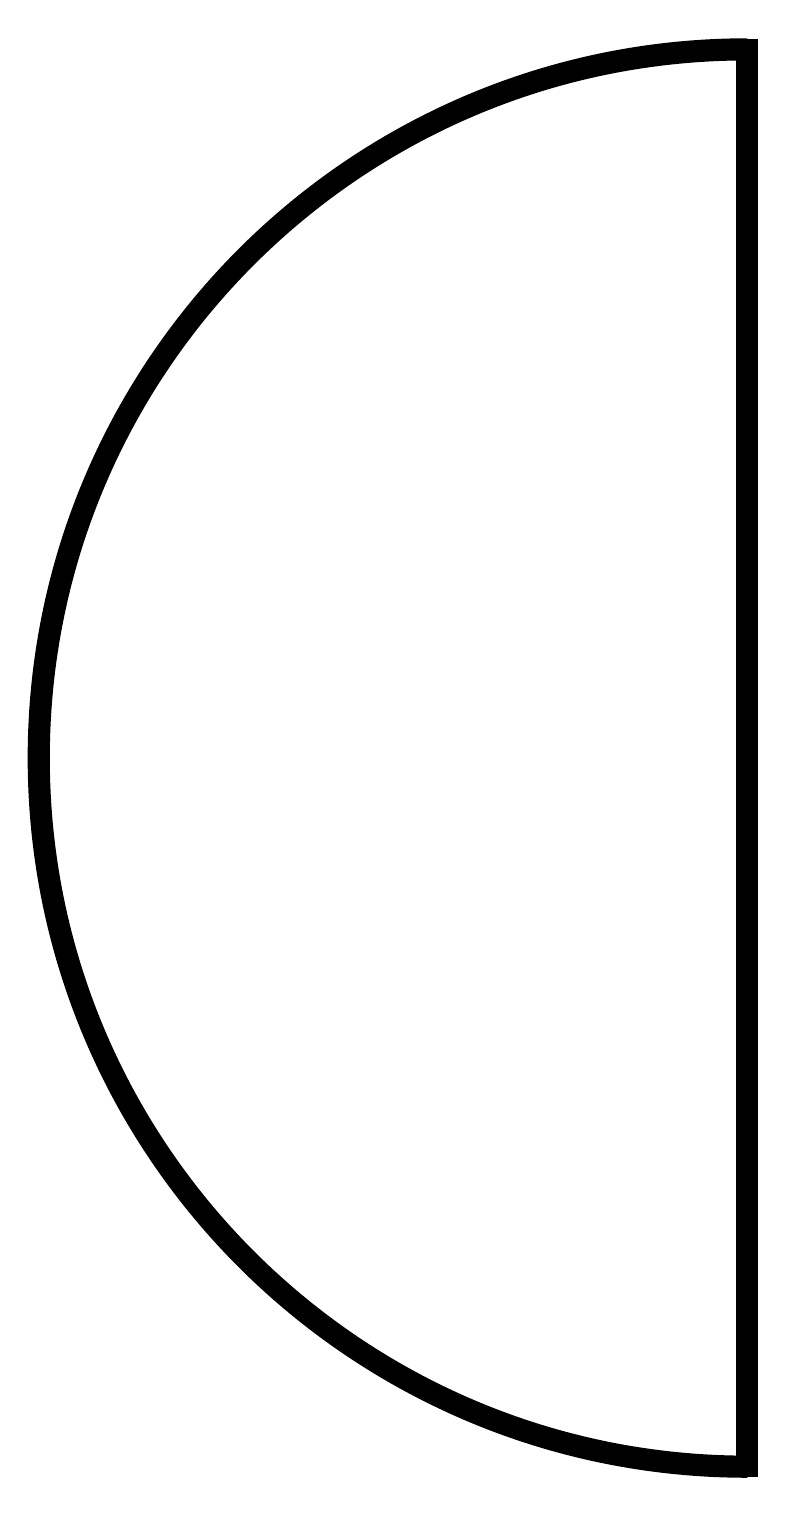
\begin{tikzpicture}

  % Bounding box of the scheme
  \draw (-4,0) node (Bb1) {} ;
  \draw (0,0) node (Bb2) {} ;

  %%%%%%%%%%%%%%%%%%%%%%%%%%%%%%%%% Background of the mesh %%%%%%%%%%%%%%%%%%%%%%%%%%%%%%%%%%%%
  \draw[color=black, line width=8] (0,9) arc [start angle=90, end angle=270, x radius=9cm, y radius=9cm];
  \draw[color=black, line width=8] (0,9.135) -- (0,-9.135) ;

\end{tikzpicture}
\end{document}
